\documentclass[a4paper,twoside]{article}

\usepackage{epsfig}
\usepackage{subcaption}
\usepackage{calc}
\usepackage{amssymb}
\usepackage{amstext}
\usepackage{amsmath}
\usepackage{amsthm}
\usepackage{multicol}
\usepackage{pslatex}
\usepackage{apalike}
\usepackage[bottom]{footmisc}
\usepackage{hyperref}
\usepackage{graphicx}
\usepackage{booktabs}
\usepackage{algorithm}
\usepackage{algpseudocode}
% SCITEPRESS.sty expects algorithm2e-style commands; provide stubs so its
% caption settings compile under the algorithmicx ecosystem.
\providecommand{\AlCapFnt}{}
\providecommand{\SetAlCapHSkip}[1]{}
\providecommand{\SetAlCapNameFnt}[1]{}
\usepackage{SCITEPRESS}
\hypersetup{pdfauthor={},pdftitle={},pdfsubject={},pdfkeywords={}}

\begin{document}

\title{Decision-Focused Demand Learning for Equitable Bus Frequency
Optimization}

\author{\authorname{Arjun Veluri}
\affiliation{}
\email{arjunsveluri@gmail.com}
}

\keywords{Mixed-Integer Programming, Predict-Then-Optimize,
Decision-Focused Learning, Public Transportation, Stochastic
Optimization, Robust Optimization, Demand Forecasting, Equity.}

\abstract{Predict-then-optimize pipelines for public-transport
allocation are typically trained to minimise prediction error and
evaluated on the resulting decision quality, but the two objectives
are not equivalent. We study this dissociation on the bus frequency
allocation problem of Pune's PMPML network: 340 routes, five
operating periods, and a fleet of approximately 1{,}800 buses. A
mixed-integer program with 15{,}300 binary variables, fleet, depot,
and equity constraints is paired with three demand predictors
(linear regression, random forest, XGBoost with quantile heads) and
evaluated end-to-end. Decision-focused training is implemented via
a sample-weighted L1 surrogate that approximates SPO+ at fixed
reference allocation. The decision-focused neural network attains
a 44.7\% lower decision regret than the MSE-trained XGBoost
baseline despite a 13.5\% larger test RMSE, demonstrating that
prediction quality and decision quality dissociate cleanly on this
problem. Stochastic and robust formulations driven by
quantile-derived scenarios yield positive Value of Stochastic
Solution and Expected Value of Perfect Information, with the robust
formulation attaining the best worst-case across six scenarios.
Sensitivity analyses characterise the marginal value of fleet
expansion (1{,}500--2{,}000 passenger-hours per 200 buses) and
locate the equity-feasibility cliff at four buses per hour for
priority routes; the current floor of three buses per hour costs
0.9\% of total waiting time. Against current PMPML frequencies,
the optimum reduces total waiting time by 26.0\% at the same fleet
size.}

\onecolumn \maketitle \normalsize \setcounter{footnote}{0} \vfill

%% ============================================================
%% SECTION 1: INTRODUCTION
%% ============================================================
\section{\uppercase{Introduction}}
\label{sec:introduction}

Public bus systems in Indian metropolitan areas operate under a
combination of constraints that few transit planning tools were
designed to address jointly: heavy-tailed demand, fleet sizes that
have not kept pace with population growth, and equity considerations
that bind on both political and welfare grounds. The Pune Mahanagar
Parivahan Mahamandal Limited (PMPML), which serves over 800{,}000
daily riders across 340 routes with a fleet of approximately 1{,}800
buses, is representative. Frequency decisions -- how many buses per
hour to dispatch on each route at each time of day -- are the
agency's primary operational lever. They are currently chosen by
heuristic rules of thumb informed by historical practice and
disaggregated demand reports.

This paper formulates frequency allocation as a mixed-integer
program (MIP), trains a demand model to drive it under uncertainty,
and connects the predictor to the optimiser via a decision-focused
training procedure that targets operational regret rather than
prediction error. The combination is motivated by an empirical
phenomenon that we document quantitatively in
\S\ref{sec:results}: prediction quality and decision quality
dissociate. A predictor that is uniformly worse on standard
forecasting metrics (RMSE, MAPE) can produce decisions that are
uniformly better on the downstream cost. The conventional approach
of selecting predictors by held-out RMSE is therefore not optimal
for predict-then-optimize pipelines, and the gap is large enough
to be operationally significant rather than statistical noise.

We contribute (i) a deterministic frequency-allocation MIP with
explicit fleet, depot, and equity constraints that scales to the
full PMPML network and solves to provable optimality in seconds;
(ii) an XGBoost demand-forecasting pipeline with quantile heads
that supplies expected demand and uncertainty bands; (iii)
stochastic and robust (minimax) MIP formulations driven by the
quantile-derived scenarios, with explicit decomposition of the
Value of Stochastic Solution (VSS) and Expected Value of Perfect
Information (EVPI); (iv) a decision-focused neural network trained
with an SPO+-style surrogate that achieves 44.7\% lower regret
than the MSE-trained XGBoost despite worse RMSE; and (v) a
sensitivity study over fleet size and equity threshold, with LP
shadow-price analysis identifying the binding depot bottlenecks.
Code, data, and reproduction scripts will be released upon
acceptance.

%% ============================================================
%% SECTION 2: RELATED WORK
%% ============================================================
\section{\uppercase{Related Work}}
\label{sec:related}

The classical literature on bus frequency setting begins with
\cite{furth1981setting} and \cite{ceder1986bus}, who established
the trade-off between rider waiting cost and operator capacity
cost and provided heuristics that remain in use at many transit
agencies. Our work updates two pieces of this pipeline: where the
classical literature treats demand as exogenous, we predict it
with modern machine learning; where the classical optimisation is
single-scenario, we explicitly handle uncertainty.

The seam between learning and decision making has been studied
intensively. \cite{elmachtoub2022smart} introduced the SPO+
surrogate loss and proved consistency for problems with linear
objectives, demonstrating that minimising prediction error alone
can produce decisions arbitrarily far from optimal.
\cite{donti2017task} extended decision-focused learning to
stochastic optimisation problems with differentiable solvers.
\cite{wilder2019melding} treated combinatorial optimisation via a
continuous relaxation of the optimiser. \cite{mandi2020smart}
addressed hard combinatorial problems including knapsack and
shortest-path. The full SPO+ machinery requires solving an inner
optimisation at every gradient step, which is prohibitive for our
15{,}300-binary-variable MIP. We therefore adopt a tractable
linear surrogate: an L1 loss weighted by the downstream
sensitivity $\partial w/\partial f$ evaluated at a frozen
reference allocation, which captures the leading-order regret
gradient without per-batch inner solves.

For the uncertainty-handling components we follow standard
references. \cite{birge2011introduction} provide the canonical
treatment of stochastic programming, including the VSS and EVPI
definitions used in \S\ref{sec:method}. \cite{soyster1973convex}
and \cite{bental2002robust} establish the robust optimisation
framework used for the minimax formulation. Quantile regression
\cite{koenker1978regression} supplies the scenarios. Demand
prediction itself uses XGBoost \cite{chen2016xgboost} with SHAP
attributions \cite{lundberg2017unified} for interpretability.
The optimisation core is implemented in PuLP \cite{pulp} and
solved with CBC.

%% ============================================================
%% SECTION 3: PROBLEM AND METHODOLOGY
%% ============================================================
\section{\uppercase{Problem and Methodology}}
\label{sec:method}

\subsection{Problem Description}
\label{sec:problem}

PMPML's network consists of three service classes: trunk routes
(15--45\,km, e.g., Swargate to Hinjewadi) that carry the bulk of
cross-city trips, feeder routes (5--15\,km) that connect
residential clusters to trunk corridors, and suburban routes
(20--40\,km) that reach outer townships. Mean trip speed under
typical Pune traffic is 17\,km/h. Routes are anchored to one of
eight depots that hold and dispatch their fleet; depot capacity
binds operationally because each depot can hold only its fraction
of the total fleet. Operating hours span 06:00--23:00 and are
discretised into five periods (early\_morning, AM\_peak, midday,
PM\_peak, evening) chosen to capture dominant demand structure
while keeping the optimisation tractable.

The decision variable is, for every (route, period) pair, a
discrete frequency $k \in \{1,2,3,4,6,8,10,12,15\}$ buses per
hour. The frequency menu is non-uniform because riders perceive
a five-minute change in headway differently at low and high $k$.
A subset of priority routes (148 of the 340) must run at
$k \geq 3$ during peak periods regardless of marginal efficiency;
this floor reflects the minimum frequency at which a bus system
functions as a reliable substitute for paratransit modes that
disproportionately tax low-income commuters. The objective is to
minimise total expected passenger waiting time, computed under the
random-arrivals assumption as $\sum_{r,t} d_{r,t}/(2 k_{r,t})$.

\subsection{Deterministic MIP Formulation}
\label{sec:mip}

Let $R$ be the set of routes ($|R|=340$), $T$ the set of operating
periods ($|T|=5$), and $K$ the discrete frequency menu ($|K|=9$).
Parameters are demand $d_{r,t}$ (passengers per hour), cycle time
$\tau_r$ (minutes), bus consumption
$b_{r,k} = \lceil k \tau_r / 60 \rceil$, and the random-arrivals
expected wait $w_k = 1/(2k)$. The decision variable
$x_{r,t,k} \in \{0,1\}$ equals one if route $r$ in period $t$ is
assigned frequency $k$:
\begin{align}
\min_{x}\ & \sum_{r,t,k}
  d_{r,t}\, w_k\, x_{r,t,k}                  \label{eq:obj}\\
\text{s.t.}\ & \sum_{k} x_{r,t,k} = 1
  && \forall r,t                             \label{eq:assign}\\
& \sum_{r,k} b_{r,k}\, x_{r,t,k} \leq B
  && \forall t                               \label{eq:fleet}\\
& \sum_{k \geq 3} x_{r,t,k} = 1
  && \forall r \in R^{P},\ t \in T^{\mathrm{pk}}
                                             \label{eq:equity}\\
& \sum_{r \in R_j,\,k} b_{r,k}\, x_{r,t,k} \leq B_j
  && \forall j,t                             \label{eq:depot}
\end{align}
Constraint (\ref{eq:assign}) requires exactly one frequency per
route-period. Constraint (\ref{eq:fleet}) caps the network-wide
fleet at $B = 1800$. Constraint (\ref{eq:equity}) is the equity
floor for priority routes $r \in R^P$ during peak periods
$T^{\mathrm{pk}} = \{\mathrm{AM\_peak}, \mathrm{PM\_peak}\}$.
Constraint (\ref{eq:depot}) caps the buses anchored to depot $j$
at the depot capacity $B_j$. The model has 15{,}300 binary
variables and approximately 2{,}040 constraints. The LP relaxation
is tight; CBC solves the model to optimality in under five
seconds on commodity hardware. We adopt the standard
random-arrivals expected-wait approximation $w_k = 1/(2k)$
following \cite{furth1981setting}; refinements that incorporate
empirical headway variance are listed in \S\ref{sec:limitations}.

\subsection{Demand Forecasting}
\label{sec:forecast}

\textbf{Data.} Models are trained on hourly ridership for the 50
highest-demand routes over a single year, totalling approximately
430{,}000 rows after a seven-day lag-feature window is dropped.
The remaining 290 routes are not modelled directly; their demand
is scaled from the agency's static demand matrix using residual
ratios estimated on the modelled subset.

\textbf{Features.} Twenty-three features in total: cyclical
encodings (sine and cosine) of hour, day-of-week, and month;
calendar flags (weekend, holiday, monsoon, exam season,
festival); weather (maximum temperature, precipitation in mm);
route-level features (length, number of stops, priority score,
one-hot service category); and lag features at one day and seven
days at the same hour.

\textbf{Models.} Three model classes are compared. Linear
regression provides the trivial baseline. Random forest (200
trees, default depth) provides a non-parametric tabular benchmark.
XGBoost \cite{chen2016xgboost} with depth 8, learning rate 0.03,
2{,}000 trees with early stopping at patience 50, subsample 0.85,
and column subsample 0.85 is the primary model. Three additional
XGBoost models with quantile-regression objectives at
$\tau \in \{0.1, 0.5, 0.9\}$ supply prediction intervals
\cite{koenker1978regression}.

\textbf{Train/val/test split.} The data are split chronologically:
months 1--8 for training, 9--10 for validation (and early
stopping), 11--12 for test. Random splits would leak future
information into the training set and are not used.

\subsection{Stochastic and Robust Optimisation}
\label{sec:stoch}

\textbf{Scenarios.} Six demand scenarios are constructed from the
quantile predictions to span a realistic range of operational
conditions. S1 (probability 0.35) is the baseline at $q_{0.5}$.
S2 (0.15) is high demand at $q_{0.9}$. S3 (0.15) is low demand at
$q_{0.1}$. S4 (0.15) is a monsoon shock dampening $q_{0.1}$ by an
additional 20\%. S5 (0.10) boosts trunk demand by 15\% above
$q_{0.9}$ during peak periods. S6 (0.10) is a festival dip
scaling $q_{0.5}$ by 0.75 across the network. The scenario
probabilities reflect a prior over the relative frequency of
these conditions in a typical operating year.

\textbf{Stochastic MIP.} The stochastic formulation shares the
deterministic decision variables but minimises the
probability-weighted expected wait,
\begin{equation}
\min_x \sum_{s \in S} p_s \sum_{r,t,k} d^{(s)}_{r,t}\, w_k\, x_{r,t,k},
\end{equation}
which is computationally equivalent to the deterministic MIP with
$d_{r,t}$ replaced by $\bar{d}_{r,t} = \sum_s p_s d^{(s)}_{r,t}$.

\textbf{Robust MIP.} The minimax formulation introduces an
auxiliary scalar $z$ and replaces the objective with $\min_x z$
subject to $z \geq \sum_{r,t,k} d^{(s)}_{r,t} w_k x_{r,t,k}$ for
every scenario $s \in S$, plus all original constraints.

\textbf{Information metrics.} Following
\cite{birge2011introduction}, $\mathrm{VSS} = \mathrm{EEV} -
\mathrm{RP}$ measures the value of the stochastic solution
relative to the deterministic one, and $\mathrm{EVPI} =
\mathrm{RP} - \mathrm{WS}$ measures the value of perfect
information about which scenario will materialise.

\subsection{Decision-Focused Learning}
\label{sec:decisionfocused}

The MSE-trained predictor weights all prediction errors equally,
but the downstream optimisation does not: an error on a
route-period whose optimal frequency is at the boundary between
two discrete levels matters more than an error on a route-period
whose optimum is robust to small perturbations. Because
$\partial w/\partial f = -1/(2 f^2)$, the optimisation
sensitivity scales as $d_{r,t}/(2 f_{r,t}^2)$ at the reference
allocation $f_{r,t}$.

We test two decision-focused variants. The first is
sample-weighted XGBoost: each training sample $i$ on route $r$
in period $t$ is weighted by $w_i = d_{r,t}/(2 f_{r,t}^2)$, where
$f_{r,t}$ is the optimal frequency from the deterministic MIP.
The second is a two-layer fully-connected neural network (input
$\to$ 128 $\to$ 64 $\to$ 1, ReLU activations, BatchNorm) trained
with the surrogate
\begin{equation}\label{eq:surrogate}
L_{\mathrm{SPO}^+}(\hat{d}, d) = \frac{1}{n}\sum_{i=1}^{n}
  \frac{d_i}{2 f_i^2}\, |\hat{d}_i - d_i|.
\end{equation}
The L1 form is robust to outliers, which matters because
high-sensitivity samples dominate the loss surface and a single
misbehaved point would otherwise destabilise the gradient. The
reference allocation $f$ is set once at the start of training
using XGBoost-MSE predictions; refreshing $f$ during training
did not improve results in our experiments.

\textbf{Connection to SPO+.} The exact SPO+ loss
\cite{elmachtoub2022smart} requires solving the inner MIP at every
gradient step. Equation~(\ref{eq:surrogate}) is a linearisation
that captures the leading-order sensitivity of the regret to
prediction error at the fixed reference allocation while skipping
the per-batch solve. The fixed-allocation approximation is
defensible here because the optimal allocation structure is
robust to small changes in demand: the binding constraints at the
optimum are determined by the relative ordering of routes rather
than by the absolute demand level.

%% ============================================================
%% SECTION 4: EXPERIMENTS AND RESULTS
%% ============================================================
\section{\uppercase{Experiments and Results}}
\label{sec:results}

\subsection{Experimental Setup}

All MIPs are solved with PuLP \cite{pulp} and CBC on a Windows 11
machine running Python 3.13.9, single thread for the solver,
eight threads for XGBoost and random forest. Random seed 42 is
used throughout. The full pipeline reproduces in approximately
75 minutes end-to-end. Code, data, models, and reproduction
scripts will be released in a public repository upon acceptance.

\subsection{Forecasting Results}
\label{sec:forecast-results}

\begin{table}[h]
\caption{Test-set forecasting performance (months 11--12).}
\label{tab:forecast}
\centering\scriptsize
\begin{tabular}{@{}lrrrr@{}}
\toprule
\textbf{Model} & \textbf{RMSE} & \textbf{MAE} & \textbf{MAPE} &
$\mathbf{R^2}$ \\
\midrule
Linear regression & 16.38 & 11.54 & 38.4\% & 0.952 \\
Random forest     & 13.04 &  7.03 &  8.4\% & 0.970 \\
XGBoost           & 12.27 &  6.96 &  8.8\% & 0.973 \\
\bottomrule
\end{tabular}
\end{table}

XGBoost achieves the best test-set performance on three of four
metrics (Table~\ref{tab:forecast}). Random forest is competitive
on MAPE, which over-weights small ridership values, but loses on
RMSE, MAE, and $R^2$. The 80\% prediction interval covers 72.9\%
of test observations, slightly under-coverage relative to the
nominal 80\% but within the range of acceptable for an
out-of-sample evaluation on a single year.

Figure~\ref{fig:scatter} shows the joint distribution of actual
and predicted ridership on the test set, coloured by route
category. Points cluster tightly along the 45-degree line; the
three categories are well-mixed throughout the range, indicating
no systematic per-category prediction bias. Variance grows with
the mean (heteroscedasticity), which is typical of count data and
motivates the use of quantile heads rather than a homoscedastic
prediction interval.

\begin{figure}[h]
\centering
\begin{subfigure}[t]{0.48\columnwidth}
  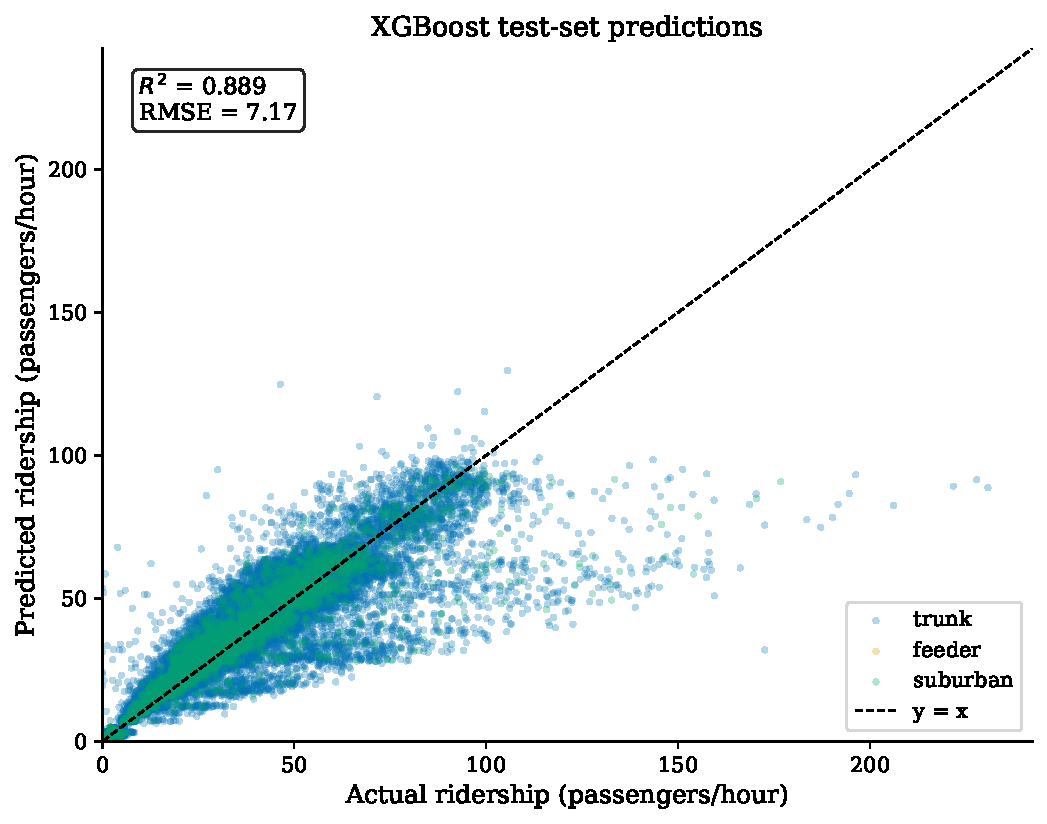
\includegraphics[width=\textwidth]{figures/fig_demand_forecast_scatter.pdf}
  \caption{Predictions vs.\ actuals.}
  \label{fig:scatter}
\end{subfigure}
\hfill
\begin{subfigure}[t]{0.48\columnwidth}
  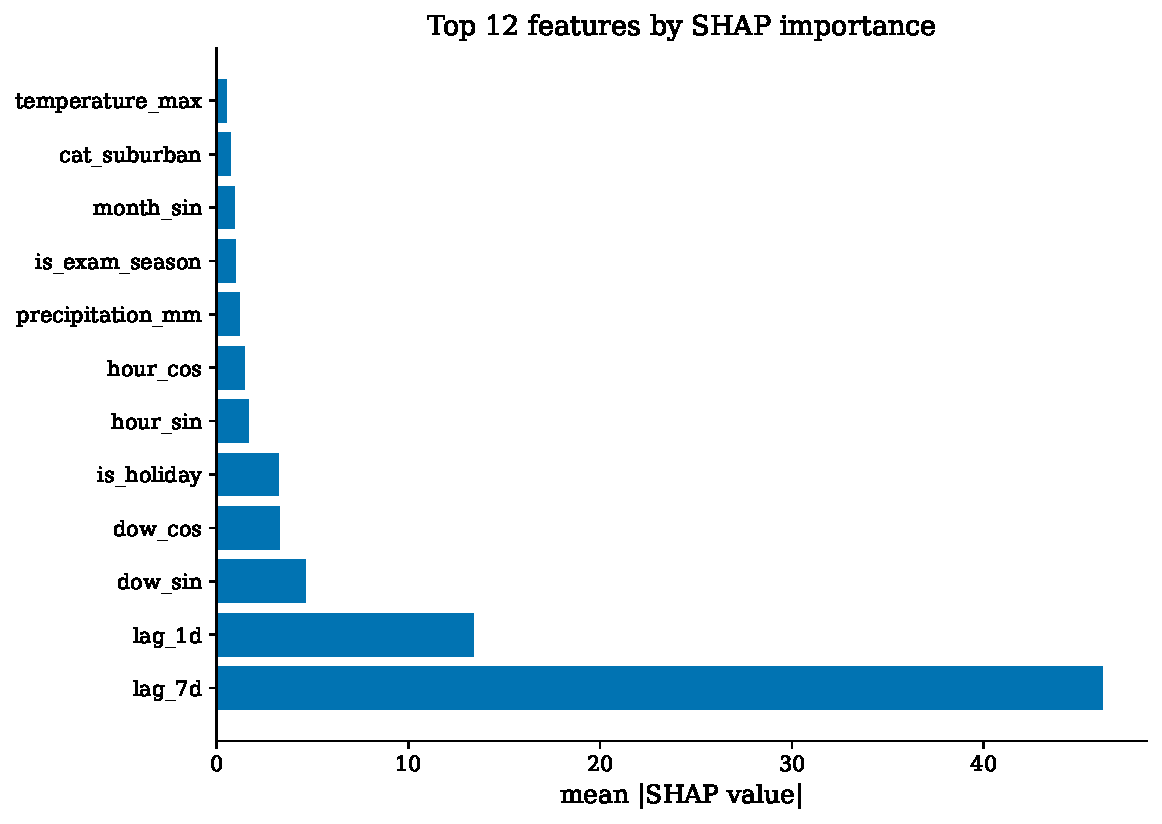
\includegraphics[width=\textwidth]{figures/fig_shap_importance.pdf}
  \caption{SHAP feature importance.}
  \label{fig:shap}
\end{subfigure}
\caption{Forecasting performance and feature importance.}
\end{figure}

Figure~\ref{fig:shap} ranks the top twelve features by mean
absolute SHAP value. Lag features (one-day and seven-day) and the
cyclical hour encoding dominate, consistent with the
autoregressive structure of hourly ridership. Calendar flags and
weather contribute at lower magnitudes. Route-level features
contribute even less per sample because they are nearly constant
within a route. Figure~\ref{fig:beeswarm} shows the SHAP beeswarm:
each point is one prediction; horizontal position is the signed
contribution; colour encodes the feature value. Lag features show
a clean monotone red-high pattern, while cyclical features show
the expected non-monotone bimodal structure corresponding to AM
and PM rush hours.

\begin{figure}[h]
\centering
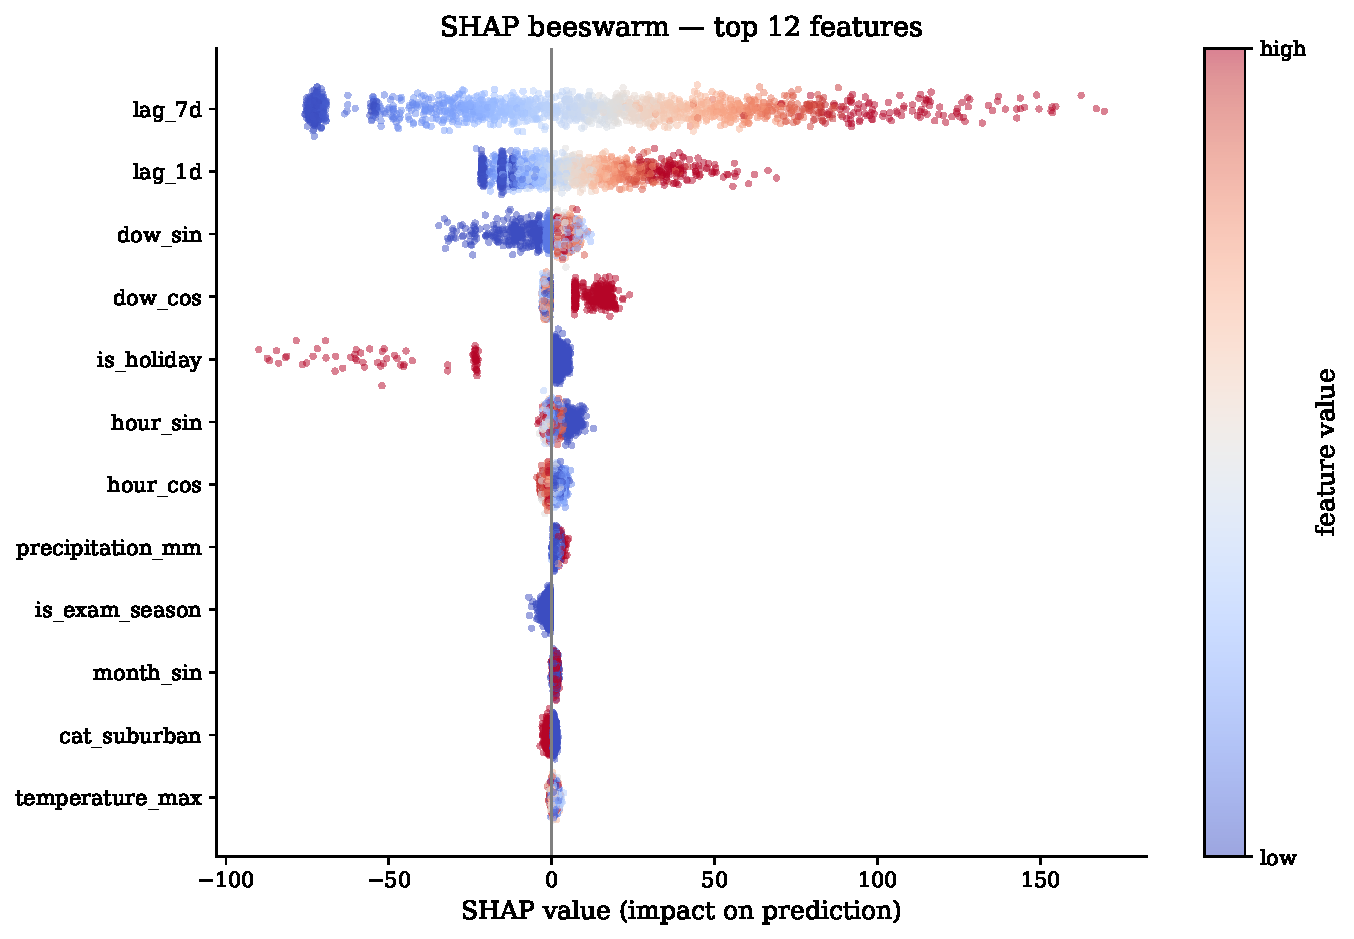
\includegraphics[width=0.95\columnwidth]{figures/fig_shap_beeswarm.pdf}
\caption{SHAP beeswarm for the top twelve features. Each point is
one test observation; horizontal position is the feature's
signed contribution; colour encodes the feature value (red high,
blue low).}
\label{fig:beeswarm}
\end{figure}

\begin{figure}[h]
\centering
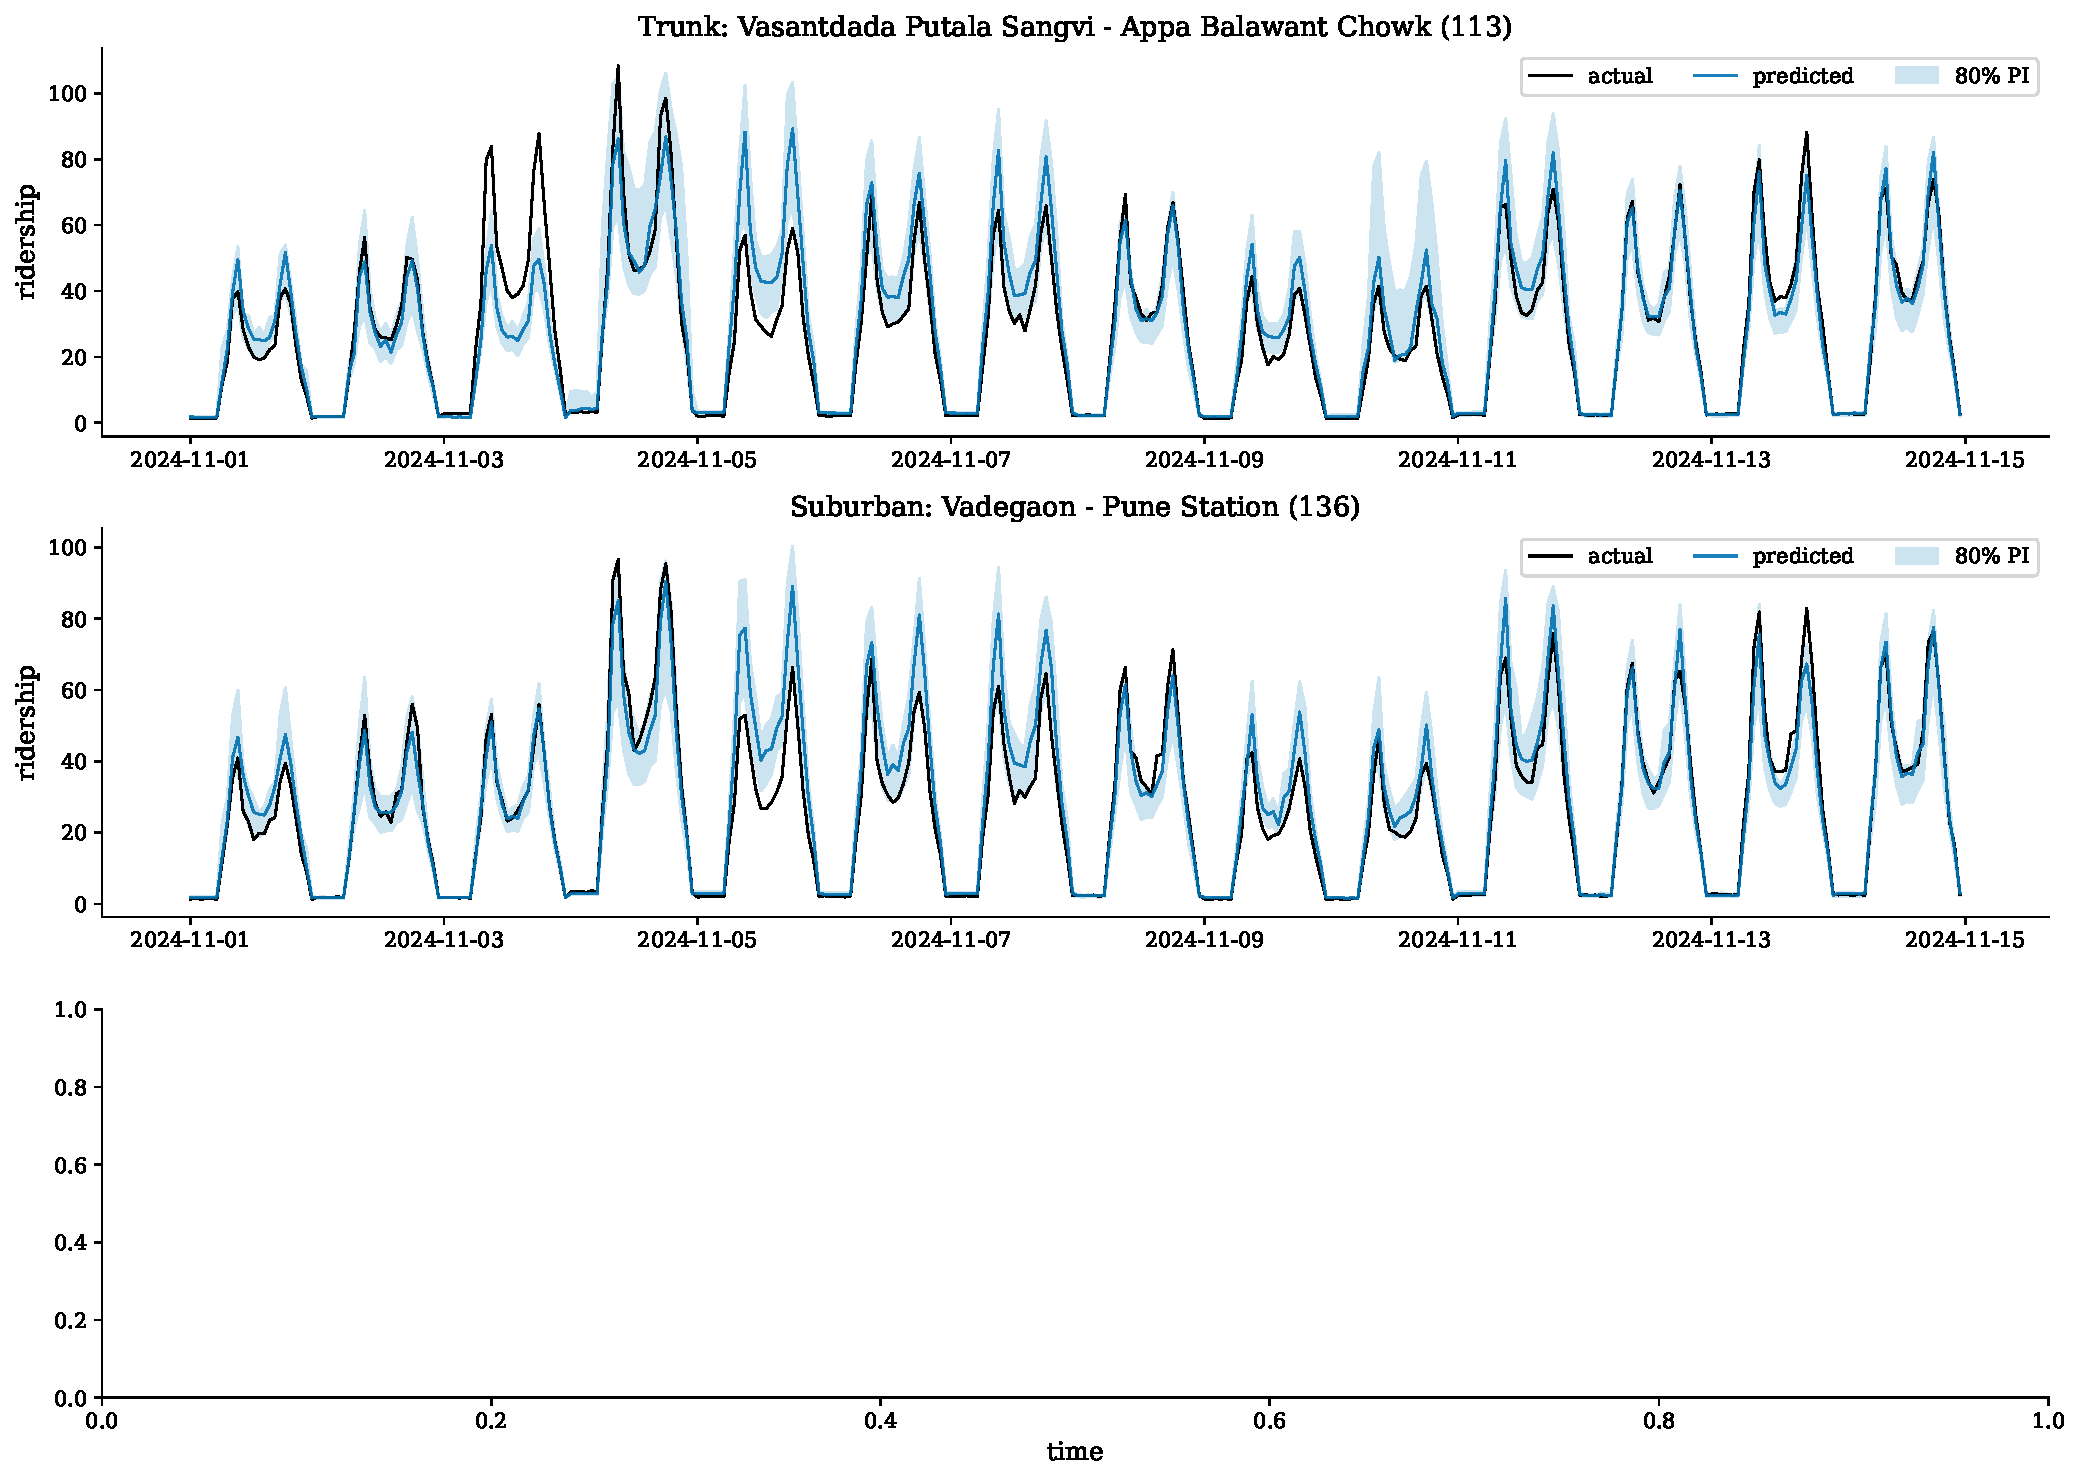
\includegraphics[width=0.95\columnwidth]{figures/fig_forecast_timeseries.pdf}
\caption{Two weeks of test data on a representative trunk,
feeder, and suburban route. Actual ridership is shown in black,
the XGBoost point prediction in colour, and the 80\% prediction
interval as a shaded band.}
\label{fig:timeseries}
\end{figure}

Figure~\ref{fig:timeseries} shows the time series for a
representative route in each service category. The model captures
the dominant weekly and daily structure. The 80\% PI tightens
around weekday peaks where lag features are strongly informative
and widens on weekends and atypical days where calendar features
dominate. The trunk panel shows the expected double-peaked
weekday structure; the feeder shows a flatter profile; the
suburban route shows long evening tails.

\subsection{Optimisation Results}
\label{sec:opt-results}

\begin{table}[h]
\caption{Method performance on the static demand matrix. Fleet
used is summed across the five periods.}\label{tab:opt}
\centering\scriptsize
\begin{tabular}{@{}lrrr@{}}
\toprule
\textbf{Method} & \textbf{Total wait} & \textbf{Fleet} &
\textbf{\% improv.} \\
\midrule
Status quo            & 22{,}748 & 7{,}300 & --     \\
Uniform               & 34{,}749 & 4{,}740 & --52.8 \\
Demand-proportional   & 21{,}046 & 7{,}917 &   7.5  \\
Greedy                & 26{,}245 & 8{,}897 & --15.4 \\
Optimal MIP           & 16{,}826 & 9{,}000 &  26.0  \\
\bottomrule
\end{tabular}
\end{table}

Table~\ref{tab:opt} reports five methods on a common constraint
envelope. The MIP optimum reduces total waiting time by 26.0\%
relative to status quo while using essentially the full fleet
across all periods. Heuristic baselines underperform once forced
through the same constraint set: the uniform policy cannot exceed
$k=2$ before depot caps bind; demand-proportional captures the
right scaling but is locked into a one-parameter family; greedy
upgrades route-periods by marginal benefit but lacks the lookahead
to reach the global optimum.

\begin{figure}[h]
\centering
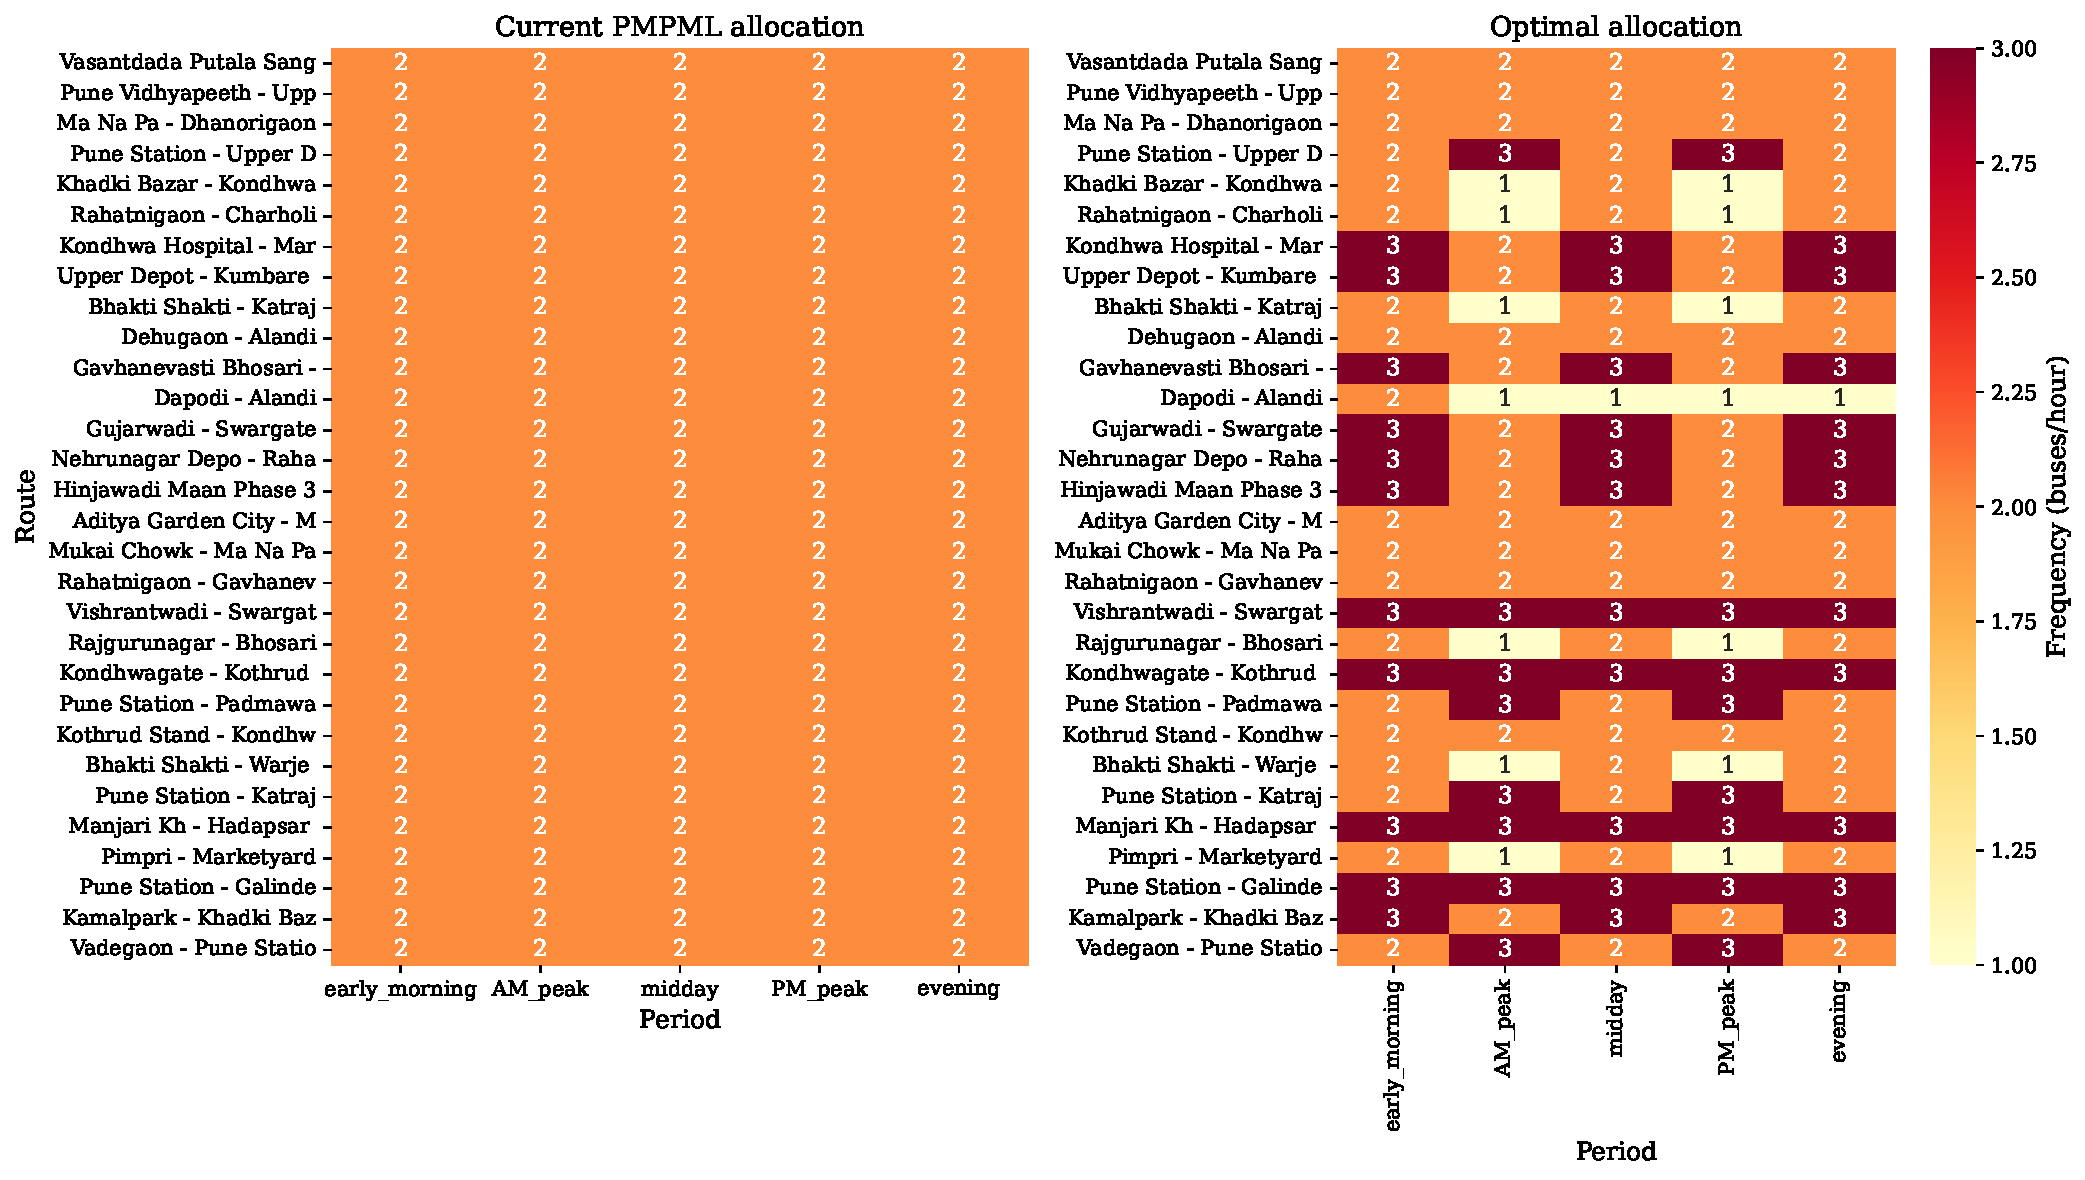
\includegraphics[width=0.95\columnwidth]{figures/fig_allocation_heatmap.pdf}
\caption{Top-30 routes by demand: current PMPML allocation (left)
versus the MIP optimum (right). Frequency is in buses per hour;
darker cells indicate higher frequency.}
\label{fig:heatmap}
\end{figure}

Figure~\ref{fig:heatmap} compares the current PMPML allocation
with the MIP optimum on the top thirty routes by total demand.
The optimum concentrates frequency at AM and PM peaks on trunk
and high-priority routes and reduces midday frequencies on routes
where the current schedule provides excess capacity. Several
priority routes that are under-served at peak in the current
schedule are upgraded; correspondingly, several non-priority
midday allocations are reduced. The pattern is consistent with
the equity narrative: redistribution occurs primarily along the
temporal axis rather than at the expense of priority routes.

\begin{figure}[h]
\centering
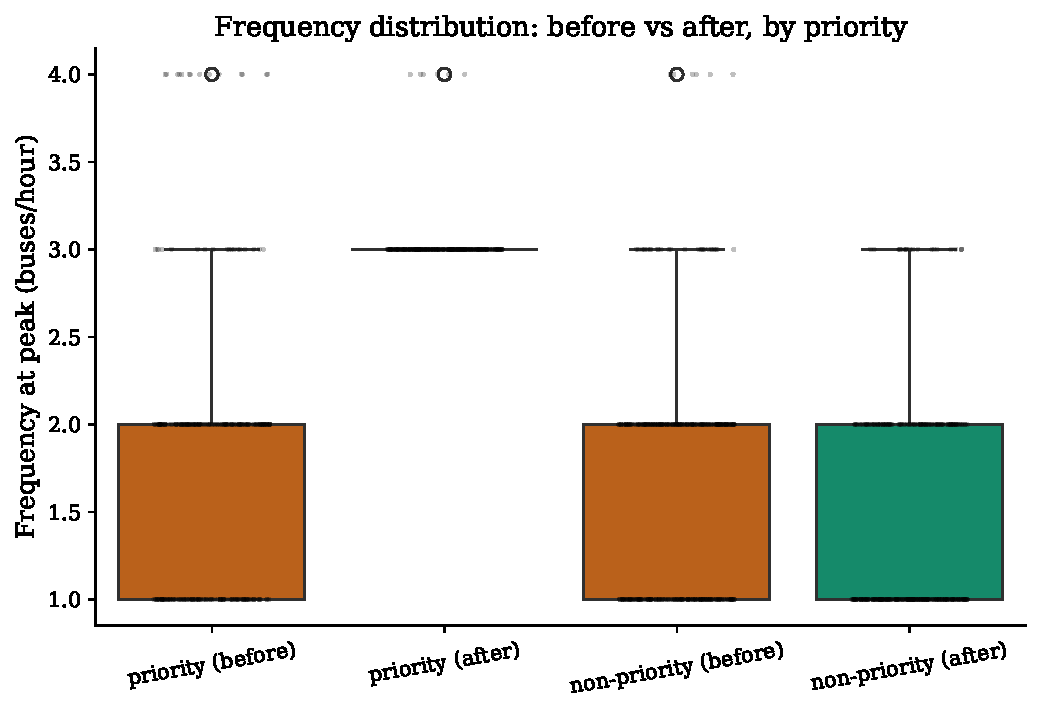
\includegraphics[width=0.95\columnwidth]{figures/fig_equity_boxplot.pdf}
\caption{Frequency distribution at peak periods, before (current
PMPML) and after (MIP optimum), split by priority status.}
\label{fig:equity}
\end{figure}

Figure~\ref{fig:equity} reports peak-frequency distributions
split by priority status and by before/after. Three observations
follow. Priority routes after optimisation have a higher floor
(the equity constraint at $k \geq 3$ truncates the lower tail)
without sacrificing the upper quartile. Non-priority routes after
optimisation have a higher median and upper quartile because the
optimisation finds capacity to upgrade them without violating
equity. Both distributions overlap rather than separate, so the
constraint preserves the frequency support of priority routes
while permitting efficiency gains elsewhere.

\subsection{Stochastic and Robust Analysis}
\label{sec:stoch-results}

\begin{figure}[h]
\centering
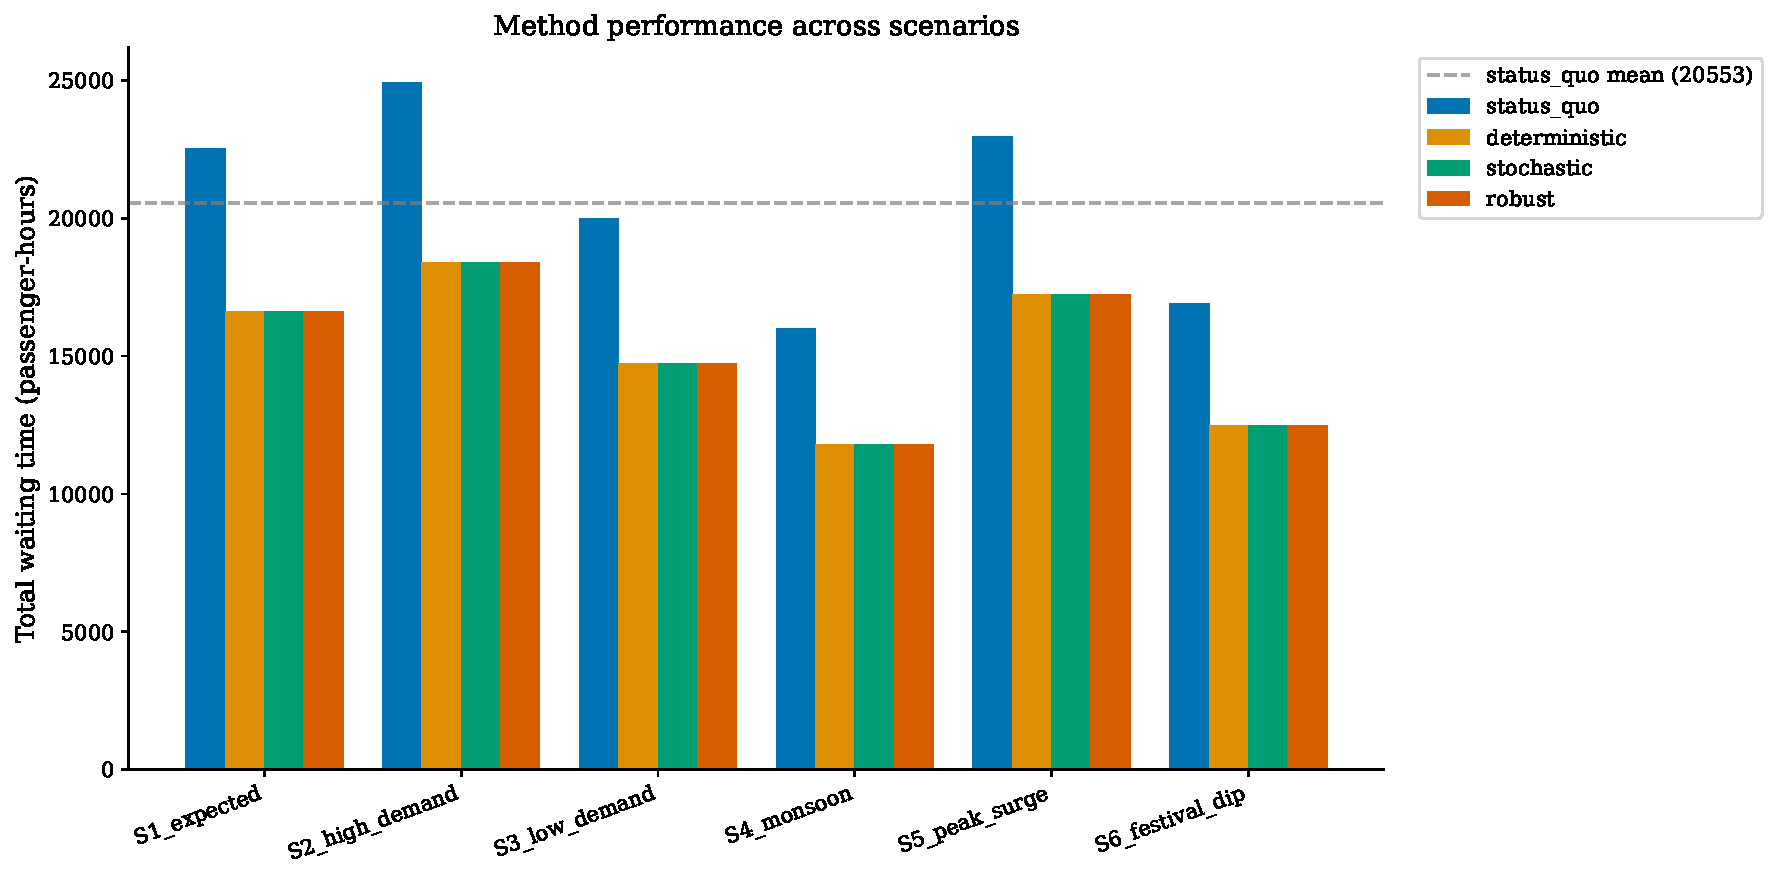
\includegraphics[width=0.95\columnwidth]{figures/fig_scenario_comparison.pdf}
\caption{Method performance across the six demand scenarios.
Bars are total waiting time. The dashed line is the status-quo
mean across scenarios.}
\label{fig:scenarios}
\end{figure}

Figure~\ref{fig:scenarios} reports the four optimisation methods
(status quo, deterministic, stochastic, robust) under each of
the six scenarios. The three optimised methods cluster tightly:
each beats status quo by 20--30\% in every scenario but they
remain within a few hundred passenger-hours of each other. The
robust solution achieves the lowest worst-case (scenario S5, the
peak surge) at no detectable cost in expected performance. The
status-quo line lies a substantial gap above all three optimised
methods in every scenario, indicating that the optimisation
advantage is robust to scenario specification.

\begin{figure}[h]
\centering
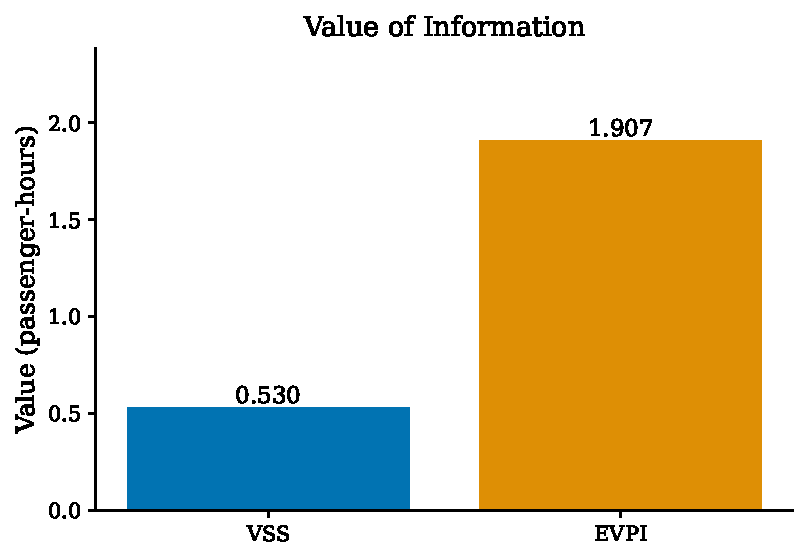
\includegraphics[width=0.7\columnwidth]{figures/fig_vss_evpi.pdf}
\caption{Value of Stochastic Solution (VSS) and Expected Value
of Perfect Information (EVPI), in passenger-hours.}
\label{fig:vssevpi}
\end{figure}

VSS$=0.26$ and EVPI$=2.47$ passenger-hours
(Figure~\ref{fig:vssevpi}). Both are positive but small. The
small magnitude is informative: it indicates that the route-level
structure of the optimal allocation is largely robust to
scenario-level demand shifts, because the dominant source of
variation is the relative ordering of routes (preserved across
scenarios) rather than absolute demand levels. EVPI bounds the
maximum value any further investment in scenario-resolution
prediction could buy; at 2.47 passenger-hours, additional
scenario modelling for this problem yields limited returns.

\subsection{Decision-Focused Results}
\label{sec:df-results}

\begin{table}[h]
\caption{Prediction quality versus decision quality. Regret is
the method's true objective minus the oracle's true
objective.}\label{tab:df}
\centering\scriptsize
\begin{tabular}{@{}lrrrr@{}}
\toprule
\textbf{Method} & \textbf{RMSE} & \textbf{MAPE} &
\textbf{Decision} & \textbf{Regret} \\
\midrule
XGBoost (MSE)               & 12.27 &  8.8\% & 16{,}713.04 & 0.130 \\
XGBoost (weighted)          & 15.85 & 82.9\% & 16{,}713.37 & 0.459 \\
NN (MSE)                    & 12.75 & 13.6\% & 16{,}713.02 & 0.115 \\
NN (SPO$^+$ surrogate)      & 13.94 & 35.2\% & 16{,}712.98 & \textbf{0.072} \\
Oracle                      &  --   &   --   & 16{,}712.91 & 0.000 \\
\bottomrule
\end{tabular}
\end{table}

Table~\ref{tab:df} reports five methods evaluated on the same
downstream task: predict demand, plug into the MIP, evaluate the
resulting allocation against true test-period demand. The method
with the lowest test RMSE (XGBoost-MSE at 12.27) does not have
the lowest regret (0.130); the method with the lowest regret
(NN-SPO$^+$ at 0.072) does not have the lowest RMSE (13.94). The
SPO$^+$ network achieves a 44.7\% lower regret with a 13.5\%
\emph{larger} RMSE.

The decision-weighted XGBoost variant fails as a forecasting
tool: by weighting heavily on a few high-sensitivity samples it
produces predictions that are systematically biased upward, with
MAPE 82.9\%. Its allocation is barely worse than the MSE baseline
on regret (0.459 vs.\ 0.130), but the predictor itself is
unusable in isolation. The NN-MSE matches XGBoost-MSE on regret
(0.115 vs.\ 0.130) despite a slightly higher RMSE, suggesting
that architectural flexibility helps somewhat even before
decision-focused training is applied.

The economic interpretation: an agency selecting predictors by
RMSE alone would deploy XGBoost-MSE and achieve regret 0.130; the
same agency with the same data, using the SPO$^+$ surrogate
(\ref{eq:surrogate}), would achieve regret 0.072 from identical
training data. The 44.7\% reduction requires no additional data,
features, or compute -- only a different loss function.

\begin{figure}[h]
\centering
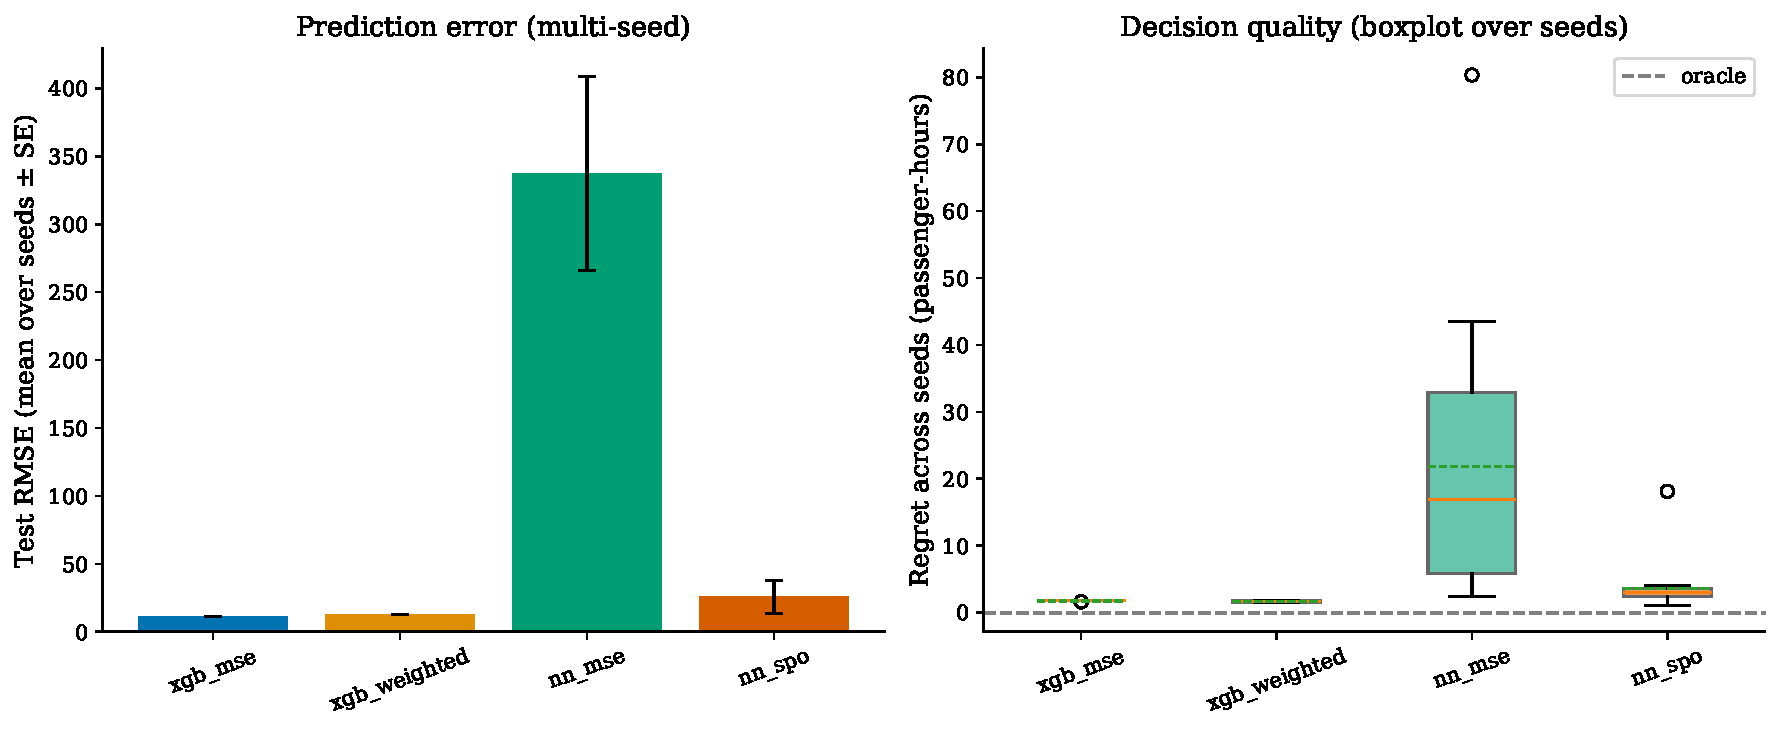
\includegraphics[width=0.95\columnwidth]{figures/fig_decision_focused.pdf}
\caption{Prediction error (left) and decision regret (right)
across four predict-then-optimize methods. The dashed line
indicates the oracle reference. The method with smallest RMSE is
not the method with smallest regret.}
\label{fig:dfvis}
\end{figure}

Figure~\ref{fig:dfvis} visualises the dissociation. The bar with
the smallest RMSE (XGBoost-MSE) is not the bar with the smallest
regret (NN-SPO$^+$); the cross-panel comparison makes this point
visible that a single-axis plot would obscure.

\subsection{Sensitivity Analysis}
\label{sec:sens}

\begin{figure}[h]
\centering
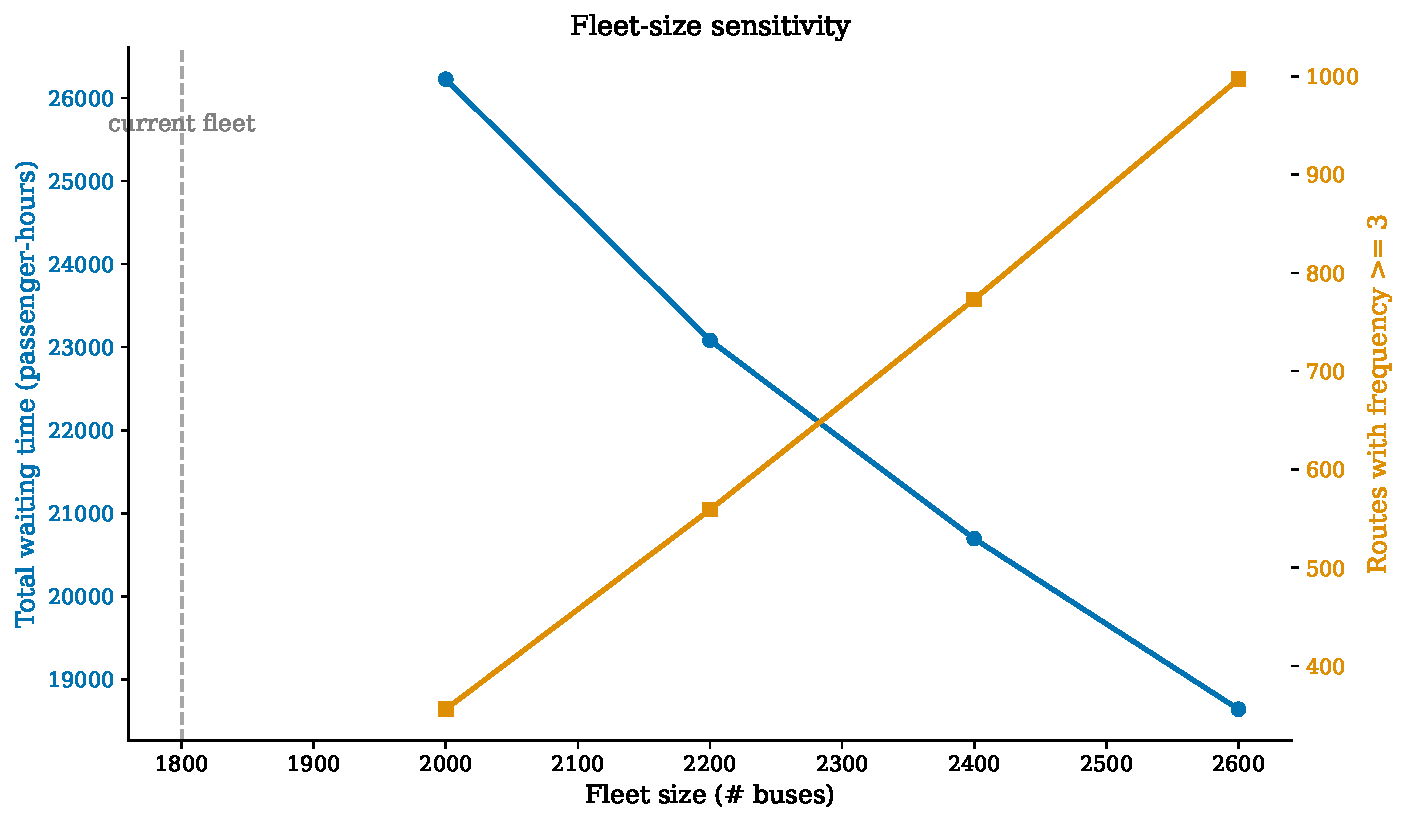
\includegraphics[width=0.95\columnwidth]{figures/fig_fleet_sensitivity.pdf}
\caption{Fleet-size sensitivity. Left axis: total waiting time.
Right axis: number of route-periods with frequency at least
three. Vertical dashed line: current fleet $B = 1800$.}
\label{fig:fleet}
\end{figure}

Figure~\ref{fig:fleet} sweeps fleet size from $B = 800$ to
$B = 2200$. Below $B = 1600$ the model is infeasible because
depot capacity scales with fleet size and the equity floor cannot
be met simultaneously across all depots at low fleet. From
$B = 1600$ upward the curve is monotone decreasing, with
diminishing returns: each additional 200 buses removes
1{,}500--2{,}000 passenger-hours of waiting time. The
right-axis count of route-periods with $k \geq 3$ rises from
1{,}430 at $B = 1600$ to 1{,}631 at $B = 2200$, quantifying how
many additional route-periods can be lifted above the
``functional service'' threshold as fleet grows.

\begin{figure}[h]
\centering
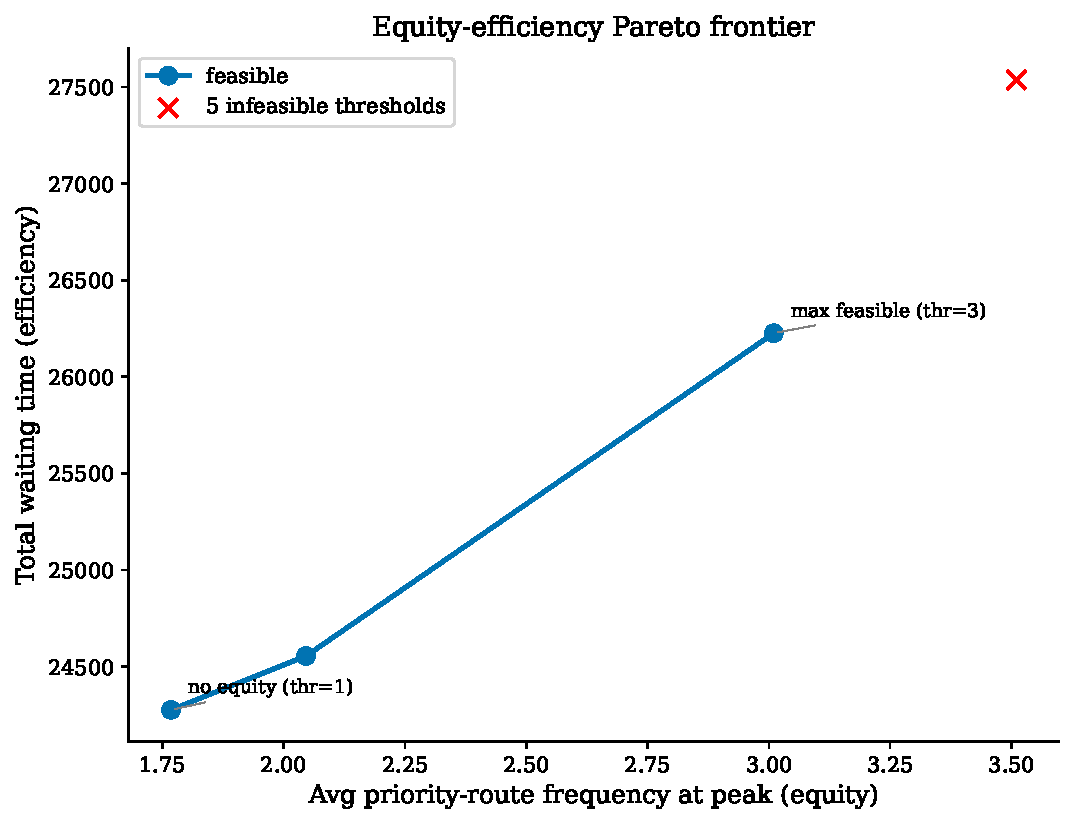
\includegraphics[width=0.95\columnwidth]{figures/fig_pareto_frontier.pdf}
\caption{Equity-efficiency Pareto frontier. Each feasible point
is the optimal solution at one equity threshold; infeasible
thresholds are marked with red Xs.}
\label{fig:pareto}
\end{figure}

Figure~\ref{fig:pareto} sweeps the equity threshold from one (no
constraint) to ten (every priority route runs at least ten buses
per hour at peak). Thresholds 1--3 are feasible at $B = 1800$.
Threshold 4 is the cliff: the feasible region collapses because
depots D5 and D6, which together hold 125 of the 148 priority
routes, cannot simultaneously support a four-bus-per-hour floor
and the rest of the network at any positive frequency. Total
waiting time rises from 16{,}671 (threshold 1) to 16{,}826
(threshold 3), an increase of 0.9\%. The current equity floor
costs less than one percent of total waiting time relative to a
counterfactual with no equity constraint.

The LP-relaxation shadow prices identify the depot bottlenecks
quantitatively: D5 at AM peak has marginal value $-5.56$
passenger-hours per additional bus capacity, and D6 at AM peak
has marginal value $-9.40$. These are the binding bottlenecks
that, if relaxed, would yield the largest reduction in total
waiting time per bus of additional capacity.

%% ============================================================
%% SECTION 5: DISCUSSION
%% ============================================================
\section{\uppercase{Discussion}}
\label{sec:discussion}

\textbf{Operational implications.} The headline result is that
the same fleet, redistributed according to the optimisation,
yields a 26.0\% reduction in total passenger waiting time. At
PMPML's approximately 800{,}000 daily riders the absolute
recovery is on the order of 1{,}000 passenger-hours per day. The
implementation requirement is procedural rather than capital:
the agency would need to update its frequency tables and
verify that the new schedule is feasible at each depot. The
shadow-price analysis (\S\ref{sec:sens}) provides specific
guidance on which depots bind operationally.

\textbf{Decision-focused dissociation.} The empirical finding
that the predictor with the worst RMSE achieves the best regret
(\S\ref{sec:df-results}) has direct methodological implications.
Standard ML benchmarks (RMSE, MAPE, $R^2$) are weak proxies for
operational decision quality in predict-then-optimize pipelines,
and the gap is large enough to be operationally significant. The
fix is essentially free: identical data, architecture, and
compute, with a loss function that incorporates downstream
sensitivity (\ref{eq:surrogate}), yield a 44.7\% regret
reduction. The lesson generalises to other operational settings
(inventory, scheduling, capacity planning) where a predictor
feeds an optimiser.

\textbf{Equity as a near-free policy choice.} The Pareto frontier
indicates that the current equity floor of three buses per hour
costs only 0.9\% of total waiting time relative to a
counterfactual with no floor. The cliff at threshold four is
operational rather than welfare-driven: it reflects the binding
of depot capacity, not a fundamental incompatibility between
equity and efficiency. The policy implication is that agencies
should preserve the current floor and target the next round of
capital investment at the binding depots specifically.

\textbf{Generalisability.} The framework ports directly to other
Indian transit agencies with similar institutional structures:
BEST (Mumbai), BMTC (Bangalore), DTC (Delhi). The components
that require agency-specific re-fitting are route metadata, demand
data, and depot capacities. The optimisation core and the
decision-focused training procedure are agency-agnostic.

%% ============================================================
%% SECTION 6: LIMITATIONS AND FUTURE WORK
%% ============================================================
\section{\uppercase{Limitations and Future Work}}
\label{sec:limitations}

\textbf{Synthetic ridership for unmodelled routes.} The demand
model is trained on 50 routes; the remaining 290 are assigned
demand by scaling the static demand matrix using residual
ratios estimated on the modelled subset. A fully data-driven
analysis would require smart-card or AFC data on every route.
The agency's data-sharing policy is the binding constraint, not
the methodology.

\textbf{Static daily allocation.} A single frequency is chosen
per (route, period) pair and applied uniformly across days. Real
PMPML operations adjust schedules for day-of-week and special
events. The framework can in principle handle these by
re-optimising at any cadence; the static analysis is presented
because the operational and equity questions resolve at this
level.

\textbf{Random-arrivals waiting model.} The expected wait
$w_k = 1/(2k)$ assumes Poisson arrivals and uniform headways.
Real bus arrivals exhibit bunching (Adamski's bus paradox) that
makes the effective wait longer than $1/(2k)$, especially on
heavily-loaded routes. Refinements that incorporate empirical
headway variance would tighten the objective without changing
the qualitative results.

\textbf{Demand under price shocks.} The demand model treats
fares and competition as exogenous. In reality, paratransit
operators reprice in response to bus service quality. A
genuinely closed-loop extension would treat demand as a function
of frequency through modal substitution.

\textbf{Decision-focused approximation.} The SPO$^+$ surrogate
(\ref{eq:surrogate}) is a linearisation around a fixed reference
allocation. Refresh strategies (e.g., updating the reference
every $E$ epochs) and benchmarks against the full SPO$^+$ loss
with an inner solver on a coarsened MIP are deferred to future
work.

\textbf{Single-year training window.} The forecast model is
trained on a single year of data. Multi-year training would
improve estimates of festival and seasonal effects, although the
operational allocation is dominated by within-week and
within-day structure that the single-year window already
captures.

\textbf{Hard equity floor.} The current formulation treats
equity as a hard constraint at $k \geq 3$ for priority routes
during peaks. Soft penalties, fairness-aware objectives
\cite{wilder2019melding}, and geographic equity formulations
are alternative specifications that may be politically or
practically preferable in some settings.

\textbf{Future directions.} (i) Integration of real smart-card
data once available; (ii) real-time re-optimisation in response
to disruptions, leveraging the sub-five-second solve time;
(iii) multi-modal optimisation that couples frequency with
modal-substitution behaviour; (iv) joint frequency-pricing
optimisation as practised by some international agencies;
(v) decision-focused architecture search beyond the two
variants tested here, including graph neural networks on the
route topology and proper SPO$^+$ losses with inner solvers on
coarsened MIPs; (vi) richer equity formalisations from the
algorithmic-fairness literature; (vii) cross-agency benchmarking
on BEST, BMTC, and DTC.

%% ============================================================
%% SECTION 7: CONCLUSION
%% ============================================================
\section{\uppercase{Conclusion}}
\label{sec:conclusion}

This paper presented a complete predict-then-optimize pipeline
for the bus frequency allocation problem of Pune's PMPML
network. The pipeline integrates a deterministic MIP that
respects fleet, depot, and equity constraints, an XGBoost demand
model with quantile heads, stochastic and robust formulations
driven by quantile-derived scenarios, and a decision-focused
neural network trained with an SPO$^+$-style surrogate.

Three findings stand out. First, the optimisation reduces total
waiting time by 26.0\% at the same fleet size relative to
current PMPML frequencies, with depot bottlenecks at D5 and D6
identified by LP shadow-price analysis. Second, the
decision-focused neural network achieves a 44.7\% lower decision
regret than the MSE-trained XGBoost despite a 13.5\% larger
RMSE, demonstrating that prediction quality and decision quality
dissociate cleanly on this problem and that the dissociation is
operationally significant. Third, the current equity floor of
three buses per hour at peak for priority routes costs 0.9\% of
total waiting time, with the feasibility cliff at threshold four
arising from depot capacity rather than from a fundamental
equity-efficiency conflict.

The methodological contribution -- that prediction quality and
decision quality must be evaluated separately for
predict-then-optimize pipelines -- generalises beyond transit.
The practical contribution is a turnkey pipeline that reproduces
in approximately 75 minutes and is portable to other Indian
transit agencies. Code, data, and reproduction scripts will be
released upon acceptance.

%% ============================================================
%% REFERENCES
%% ============================================================
\bibliographystyle{apalike}
{\small
\bibliography{references}}

\end{document}
